\documentclass{report}
\usepackage[margin=1in, paperwidth=8.5in, paperheight=11in]{geometry}
%Math packages%
\usepackage{amsmath}
\usepackage{amsthm}
%Spacing%
\usepackage{setspace}
\onehalfspacing
%Lecture number%
\newcommand{\lectureNum}{8}
%Variables - Date and Course%
\newcommand{\curDate}{January 26, 2017}
\newcommand{\course}{CS 240}
%Defining the example tag%
%\theoremstyle{definition}%
\newtheorem{ex}{Example}[section]
\newtheorem{Theorem}{Theorem}
%Setting counter given the lecture number%
\setcounter{chapter}{\lectureNum{}}
%Package to insert code%
\usepackage{listings}
\usepackage{courier}
\usepackage{xcolor}
\lstset { 
    tabsize=2,
    breaklines=true,
    language=C++,
    backgroundcolor=\color{blue!8}, % set backgroundcolor
    basicstyle=\footnotesize\ttfamily,% basic font setting
}
%Package to draw trees%
\usepackage{tikz}
\usetikzlibrary{shapes}
\begin{document}
%Note title%
\begin{center}
\begin{Large}
\textsc{\course{} | Lecture \lectureNum{}}
\end{Large}
\end{center} 
\noindent \textit{Bartosz Antczak} \hfill
\textit{Instructor: Eric Schost} \hfill
\textit{\curDate{}}
\rule{\textwidth}{0.4pt}

% Actual Notes%
\subsubsection{Bounds on Sorting}

So far, our most efficient sorting algorithm has a worst-case running
time of $\Theta(n \log n)$. Can we do better than this? Yes and no! It
depends on our computation model.


\section{The Comparison Model}
In the \textbf{comparison model}, data can only be accessed in two ways:
\begin{itemize}
\item Comparing two elements
\item Moving elements around (i.e., copying, swapping)
\end{itemize}
All of the algorithms we've seen so far are in the comparison model.

\begin{Theorem}
{Any correct comparison-based sorting algorithm requires at least $\Omega(n \log n)$ comparison operations}
\end{Theorem}

\begin{proof}
An algorithm can be viewed as a \textit{decision tree}, where each
internal node is a comparison. For instance, the following algorithm
sorts arrays of length 2:

\begin{lstlisting}
Sort-2Array(A){
  if (A[0] > A[1]){
    swap(A[0], A[1])
  }
}
\end{lstlisting}
It can be represented by the following decision tree
\begin{center}
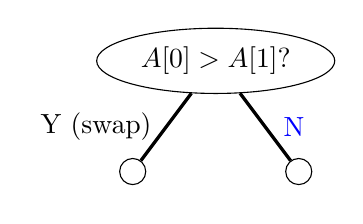
\begin{tikzpicture}[
  edge from parent/.style={very thick,black,draw},
  level distance=40 pt,
  every node/.style={circle,draw},
  level 1/.style={sibling distance=60 pt},
  level 2/.style={sibling distance=60 pt},
]
  \node[ellipse] {$A[0] > A[1]$?}
    child {node{~} edge from parent node[left,draw=none]{Y (swap)}}
    child {node{~} edge from parent node[right,draw=none,blue]{N}}
    ;
\end{tikzpicture}
\end{center}
On input $[1,2]$, we take the path N (in blue) from the root; on input $[2,1]$,
we take the path Y (black). In particular, the number of leaves (2) is the number 
of possible permutations of $[1,2]$.

Now, consider the following algorithm for arrays of length 3.
\begin{lstlisting}
Sort-3Array(A){
  if (A[0] > A[2]){
    swap(A[0], A[2])
  }
  if (A[1] > A[2]){
    swap(A[1], A[2])
  }
  if (A[0] > A[1]){
    swap(A[0], A[1])
  }
}
\end{lstlisting}
It can be represented by the following decision tree
\begin{center}
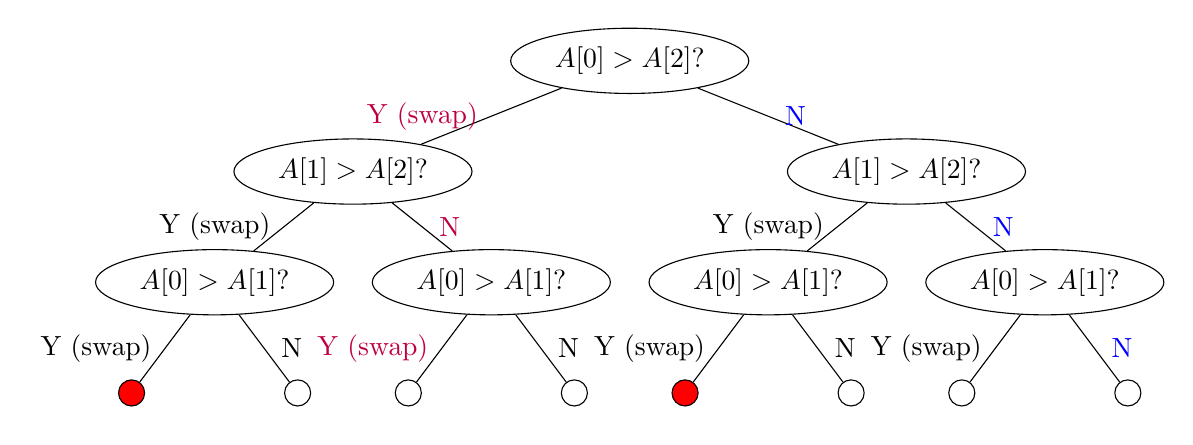
\begin{tikzpicture}[
  level distance=40 pt,
  every node/.style={circle,draw},
  level 1/.style={sibling distance=200 pt},
  level 2/.style={sibling distance=100 pt},
  level 3/.style={sibling distance=60 pt},
]
  \node[ellipse] {$A[0] > A[2]$?}
    child {
      node[ellipse]{$A[1]>A[2]$?}
      child{
        node[ellipse]{$A[0]>A[1]$?}
        child{
          node[fill=red]{~} edge from parent node[left,draw=none]{Y (swap)}
        }
        child{
          node{~} edge from parent node[right,draw=none]{N}
        }
        edge from parent node[left,draw=none]{Y (swap)}
        ;
      }
      child{
        node[ellipse]{$A[0]>A[1]$?}
        child{
          node{~} edge from parent node[left,draw=none,purple]{Y (swap)}
        }
        child{
          node{~} edge from parent node[right,draw=none]{N}
        }
        edge from parent  node[right,draw=none,purple]{N}
        ;
      }
      edge from parent  node[left,draw=none,purple]{Y (swap)}
      ;
    }
    child {
      node[ellipse]{$A[1]>A[2]$?}
      child{
        node[ellipse]{$A[0]>A[1]$?}
        child{
          node[fill=red]{~} edge from parent node[left,draw=none]{Y (swap)}
        }
        child{
          node{~} edge from parent node[right,draw=none]{N}
        }
        edge from parent  node[left,draw=none]{Y (swap)}
        ;
      }
      child{
        node[ellipse]{$A[0]>A[1]$?}
        child{
          node{~} edge from parent node[left,draw=none]{Y (swap)}
        }
        child{
          node{~} edge from parent node[right,draw=none,blue]{N}
        }
        edge from parent  node[right,draw=none,blue]{N}
        ;
      }
      edge from parent  node[right,draw=none,blue]{N}
      ;
    }
    ;
\end{tikzpicture}
\end{center}
On input $[1,2,3]$, we take the path NNN (in blue); on input $[3,1,2]$,
we take the path YNY (in purple). Here the number of leaves is 8, 
which is not the number of inputs (6). This is because two leaves 
are not reachable (in solid red). Once we remove them (and all branches that 
lead to them), we are left with a tree with 6 leaves, which correspond to
6 possible inputs. 

The construction generalizes to any input size; we build a tree with $n!$ 
leaves, that correspond to $n!$ permutations of $[1,\dots,n]$. The height of 
this tree is the length of the longest path root to leaf, that is, the maximum
number of comparisons the algorithm will do, over all $n!$ inputs.

To finish the proof, we will use the fact that in a binary tree of
height $h$, with $N$ nodes and $M$ leaves, we have 
$$ h \ge \log_2(N)-1 \ge \log_2(M)-1.$$
The second inequality is easy (because $N \ge M$). For the first one,
we saw (when we studied heaps) that in a binary tree of height $h$, 
the maximum number of nodes is $2^{h+1}-1$. So $N \le 2^{h+1}-1 \le 2^{h+1}$;
taking logs, we get our inequality.

Back to our decision tree. Here, we have $M=n!$ leaves, so the height
is at least $\log_2(n!)-1$, which is $\Omega(n\log(n))$.
\end{proof}

\section{Non-comparison-based Sorting: radix sort}

\subsection{Countsort}

\begin{lstlisting}
// A: array of size n containing numbers in {0, . . . , R-1}
count-sort(A) {
	// count how many numbers of each value there are
	C = array of size R, filled with zeros
	for i 0 0 to n-1 do {
		increment C[A[i]]
	}
	/* find left boundary for each kind (this is used to determine the starting index for the number of value i */
	I = array of size R, I[0] = 0
	for i = 1 to R-1 do {
		I[i] = I[i-1] + C[i-1]
	}
	// copy, then move back in sorted order
	B = copy(A)
	for i = 0 to n-1 do {
		A[I[B[i]]] = B[i]
		increment I[d]
	}
}
\end{lstlisting}

\subsection{MSD Sort}
This algorithm sorts an array of numbers in base $R$ (e.g., $R$ is most commonly 2, 10, 128, or 256) by comparing each digit of the numbers rather than the whole number itself. Before we begin the algorithm, we want to ensure that every element has the same number of digits. We achieve this by finding the number with the largest digit, and adding the remaining leading 0s to every other element in the array (e.g., \{3, 23, 4\} becomes \{03, 23, 04\}).
\begin{lstlisting}
// A: array of size n, containing m-digit numbers
// l, r, d: integers, 0 <= l, r <= n-1, 1 <=d <= m
RadixSort(A, l, r, d) {
	if (l < r) {
		// partition A[l...r] into bins according to d-th digit
		count-sort(A[l...r])
		if (d < m) {
			for (i = 0 to R-1) {
				(let li and ri be boundaries of i-th bin)
				RadixSort(A, li, ri, d+1)
			}
		}
	}
}
\end{lstlisting}
How do we sort the $R$ bins? We do so by \textit{counting}:
If the largest number of digits that an element in the array has is $m$, then the algorithm does $n$ operations, $m$ times (i.e., this algorithm has a runtime of $O(mn) = O(n)$).
%END%
\end{document}
